\documentclass{article}
\usepackage{amsmath}
\usepackage{tikz}

\begin{document}

\section*{Question}

Solve the following system of equations for \(x\) and \(y\):

\[
\begin{cases}
3x + 4y = 10 \\
2x - y = 3
\end{cases}
\]

\section*{Solution}

To solve the system of equations, we can use the method of substitution or elimination. Here, we will use the elimination method.

First, we multiply the second equation by 4 to align the coefficients of \(y\):

\[
\begin{cases}
3x + 4y = 10 \\
8x - 4y = 12
\end{cases}
\]

Next, we add the two equations to eliminate \(y\):

\[
(3x + 4y) + (8x - 4y) = 10 + 12
\]

\[
11x = 22
\]

\[
x = 2
\]

Now, substitute \(x = 2\) back into the first equation:

\[
3(2) + 4y = 10
\]

\[
6 + 4y = 10
\]

\[
4y = 4
\]

\[
y = 1
\]

Thus, the solution to the system of equations is \(x = 2\) and \(y = 1\).

\section*{Graphical Representation}

\begin{tikzpicture}[scale=1]
    \draw[very thin,color=gray] (-3.1,-3.1) grid (3.9,3.9);
    \draw[->] (-3.2,0) -- (4.2,0) node[right] {$x$};
    \draw[->] (0,-3.2) -- (0,4.2) node[above] {$y$};

    % Equation 1: 3x + 4y = 10
    \draw[blue, thick, domain=-3:4] plot (\x, {2.5 - 0.75*\x}) node[right] {$3x + 4y = 10$};

    % Equation 2: 2x - y = 3
    \draw[red, thick, domain=-3:4] plot (\x, {2*\x - 3}) node[right] {$2x - y = 3$};

    % Solution point
    \fill[black] (2,1) circle (2pt) node[above right] {$(2,1)$};
\end{tikzpicture}

% Create another example for students to work through

\section*{Question}

Solve the following system of equations for \(x\) and \(y\):

\[
\begin{cases}
2x - 3y = 5 \\
3x + 2y = 8
\end{cases}
\]

\section*{Graphical Representation} 

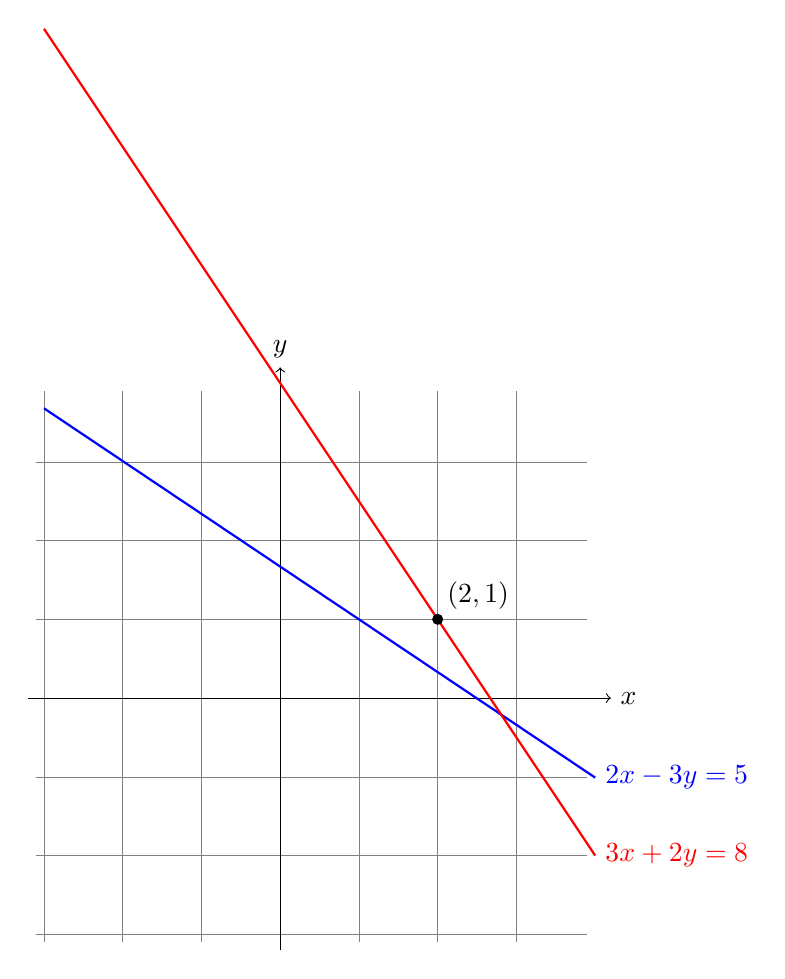
\begin{tikzpicture}[scale=1]
    \draw[very thin,color=gray] (-3.1,-3.1) grid (3.9,3.9);
    \draw[->] (-3.2,0) -- (4.2,0) node[right] {$x$};
    \draw[->] (0,-3.2) -- (0,4.2) node[above] {$y$};

    % Equation 1: 2x - 3y = 5
    \draw[blue, thick, domain=-3:4] plot (\x, {1.67 - 0.67*\x}) node[right] {$2x - 3y = 5$};

    % Equation 2: 3x + 2y = 8
    \draw[red, thick, domain=-3:4] plot (\x, {4 - 1.5*\x}) node[right] {$3x + 2y = 8$};

    % Solution point
    \fill[black] (2,1) circle (2pt) node[above right] {$(2,1)$};
\end{tikzpicture}


\end{document}